\documentclass{article}
\usepackage[utf8]{inputenc}

\title{mcm 2021}
\author{}
\date{February 2021}

\usepackage{natbib}
\usepackage{graphicx}
\usepackage{footnote}

\begin{document}
% To-do:
% -more environmental impacts (solidify model and sources, need moisture content!)
% -background on hyphal tip extension?
% -intro?
% -top level explaining
% -niches as a form of interaction
% -complementary decomposition as a form of interaction
% -advantages and disadvantages of general niches
% -short vs long term fluctuations
%     -soil hystersis and subtle effect --> shift soil profile long term
%     -short term soil profile not impacted, but temp and moisture content of ground
% -environmental model pro con
%     -3 comp: temp, water+soil comp-> water potential
%     -benefits of water potential over content alone --> allows more long terms investigation
%     -neglects interactions with non-fungal species
%     -generalizes ground as soil -> neglects roots
%     -neglects unusual water storage, such as tundra
%     -low resolution
\maketitle

\section{Environmental Impacts}

\subsection{Environmental Influence on Hyphal Tip Extension ($\nu$)}
Environmental impacts are introduced to the decomposition model through $\nu$, the hyphal tip elongation rate. This elongation occurs at tip of the hyphae via vesicles known as Spitzenkorper, but the mechanism of this extension remains unknown \cite{Steinberg2007}. As described in Gervais et al. 1999, "cell turgor pressure corresponds to an overpressure which allows the cell morphology, elongation, division and hence the biomass evolution" \cite{Gervais1999}. In fungi, cell turgor itself is respondent to water potential gradients rather than to active transport within the cell, making it very environmentally dependent \cite{Gervais1999}. Thus, we have reason to examine environmental impacts on fungal decomposition rates by varying $\nu$ outside of baselines for given species in set locations.

This brings us to the issue of determining $\nu$ based on environmental factors. Experimental data from Maynard et al. 2019 shows the relationship between $\nu$ and the environmental parameters of water potential and temperature \cite{Maynard2019}.  Water potential as a parameter will take into account both moisture content to fungi as well as the availability of that moisture as dictated by the  soil composition.

\subsection{Estimating $\nu$ For Various Environments}

When considering a sampling of decomposition rates in various environment types, we must determine how to estimate temperate and water potentials that ground fungi would experience. In the case of determining $\nu$, this requires finding projected temperature and water potential.

Amongst existing biome classification models, Whitaker's scheme \cite{whittaker1970} is perhaps the simplest, being particularly trait-based. Whitaker's scheme provides a layout of biomes based on mean annual temperature and mean annual precipitation. However, modern classification of biomes has drifted away from using these traits as definitive biome identifiers \cite{mucina2018}. These traits alone do not define all features of concern to fungal growth, such as soil composition for example. Thus, we can use a combination of Whitaker's scheme and additional profiling of the scheme to examine the advantages and disadvantages of different species in different environments. We will sample within the temperature range of Whitaker's scheme: $-15^{\circ}$ to $30^{\circ}$ C of mean annual temperature.

 Although water potentials can be approximated based on predictive models, the measure is best found experimentally from soil samples \cite{Abkenar2019}. Ranges for moisture potential of these environments have been found experimentally from a variety of studies is shown in the following table. Note that these potentials are for various seasons, as we are aiming to compare discrete environmental conditions rather than create a complete span of environmental conditions.

\begin{savenotes}
\begin{table}[ht]
\begin{center}
 \begin{tabular}{|c c c c|} 
 \hline
 Biome/ Environment & Specific Location & Water Potential [MPa] \\ [0.5ex] 
 \hline\hline
 Dessert (Arid) & Sonoran Desrt, USA & -4.0 to -5.0 MPa \cite{Nilsen1983} \\ 
 \hline
 Grasslands/shrublands (Semi-Arid) & Grasslands, central Argentina \footnote{Measurements taken November through January at 100 cm soil depth.} & -1.4 to -5.0 \cite{Pelaez 1994}\\
 \hline
 Temperate Forest & Sal Forests, central Himalayas & -0.44 (Fall) to -1.81 (Summer) \cite{Zobel2001} \\
 \hline
 Boreal Forest (Arboreal) & Pine Forests, central Himalayas & -0.83 (Fall) to -3.36 (Summer) \cite{Zobel2001}\\
 \hline
 Tropical Rain Forest & Tropical Karst Forests &  \\ [1ex] 
 \hline
\end{tabular}
\end{center}
\end{table}
\end{savenotes}

Given these estimates, we can have a probable example combination of temperature and moisture potential in various environments. Note that these are not wholly representative configurations, but rather examples to provide insight into how fungal species with specific traits may respond in discrete and distinct conditions likely to exist. 

We can then find $\nu$ using experimental data from Maynard et al 2019. ****

\subsection{Other Responses to Temperature and Water Potential}

****

\subsection{Responses to Other Environmental Parameters}
****this whoke part is chaos***
% USE FOR ANALYSIS OF HYSTERSIS ETC LATER
The mean soil profile distributions by percentage is \cite{Zhao2019} \footnote{Note that here we neglect uncertainties for these percentages, as we need only a general estimate of the biome.}: 
\begin{center}
 \begin{tabular}{|c c c c|} 
 \hline
 Biome/ Environment & Sand [\%] & Silt[\%] & Clay[\%] \\ [0.5ex] 
 \hline\hline
 Dessert (Arid) & 43.21 & 33.67 & 23.05 \\ 
 \hline
 Grasslands/shrublands (Semi-Arid) & 45.14 & 34.71 & 20.15 \\
 \hline
 Temperate Forest & 45.42 & 34.97 & 19.59 \\
 \hline
 Boreal Forest (Arboreal) & 50.01 & 32.77 & 17.22 \\
 \hline
 Tropical Rain Forest & 42.42 & 27.05 & 30.53 \\ [1ex] 
 \hline
\end{tabular}
\end{center}


To define soil characteristics of various sample biomes within Whitaker's scheme, we can refer to the sampling documented in {}, which describes soil properties found in the top 30 cm.

Thus, we will use the two aforementioned schemes to provide us with a more focused selection of the following environments, whose properties will be expanded upon:
\begin{itemize}
\item Arid: We will focus on the arid biome of an arid dry desert. We will anticipate

\item Semi-arid: We will focus on the semi-arid biome of a semi-arid. 

\item Temperate: We will focus on a temperate climate of temperate forests

\item Arboreal

\item Tropical rain forests

\end{itemize}

% while Holdridge's scheme looks at precipitation along with mean annual biotemperatures and potential evapotranspiration ratio to mean total annual precipitation
% \begin{figure}[h!]
% \centering
% 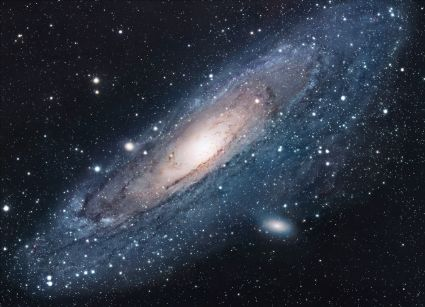
\includegraphics[scale=1.7]{universe}
% \caption{The Universe}
% \label{fig:universe}
% \end{figure}
\section{Interactions}

\subsection{Niches}

Evidence has pointed towards the development of niches in fungal communities; in particular, niches for slow growing but more resilient species of fungi vs quicker-growing but more sensitive material \cite{GUIDE ONE****}. In addition, there are specialized lignin-consuming and slow growing strains \cite{Moorhead2006}. 

\section{Model Parameters}

Here are the model parameters for the coupled decomposition and growth model for Armillaria gallica located at 30.465247 degrees latitude and -89.040298 degree longitude secreting cellobiohydrolase (Cel7A) to decompose hardwood holocellulose \cite{Maynard2019} \cite{Kari2014}:

\begin{center}
 \begin{tabular}{|c c c c c|} 
 \hline
 Parameter & Symbol & Units & Value & Source \\
 \hline\hline
 Half-Saturation Constant (Michaelis Constant) & $K_e$ & $\frac{g_{enzyme}}{L_{litter}} $ & 7 & \cite{Kari2014} Specific to Cel 7A in **** \\ 
 \hline
 Holocellulose carbon \footnote{We assume that all carbon compounds excluding lignin are holocellulose} & $LCI$ & $\frac{g}{??} $ & -.709 & \cite{Kari2014} \\ [1ex] 
 \hline
\end{tabular}
\end{center}


\bibliographystyle{plain}
\bibliography{references}
\end{document}
